\header{3}
\chapter{Veiligheid, Weer \& Vaarproblematiek}
\section{Inleiding}
Wanneer je wil gaan zeilen is het belangrijk dat dit veilig gebeurt. Om voor deze veiligheid te zorgen zijn een aantal punten van groot belang. Hierbij kan je denken aan een reddingsvest, kennis van het weer, kennis van je boot maar ook dat van andere boten. Al deze punten worden in dit hoofdstuk behandeld.
\section{Reddingsvest}
Een reddingsvest is een belangrijk onderdeel van de veiligheid aan boord. Er zijn 5 situaties waar je een reddingsvest aan moet:
\begin{enumerate}
\begin{multicols}{2}
    \item Als je boots het zegt
    \item Als de staf het zegt
    \item Als de waterpolitie het zegt 
    \item Als je het zelf wilt 
    \item Wanneer je een regenjas, regenbroek of kaplaarzen aan hebt
\end{multicols}
\end{enumerate}
Daarnaast zijn er een aantal strenge eisen aan reddingsvesten. Een reddingsvest moet:
\begin{itemize}
    \item Je binnen 15 seconden op je rug draaien
    \item Je mond 7 cm boven de het water houden
    \item De tekst \textit{``Front''} aan de voorkant bevatten
    \item In het Nederlands gegevens over het drijfvermogen en maximaal gewicht van de drager bevatten
    \item De naam en het adres van de fabrikant bevatten
    \item Voorzien zijn van handvatten waar iemand mee uit het water getild kan worden
    \item Oranje of rood zijn.
\end{itemize}

\section{Omslaan}
Wanneer je boot is omgeslagen, \textbf{blijf je bij je boot}. Het is namelijk altijd gevaarlijker om te gaan zwemmen dan om bij je boot te blijven. Hier zijn een aantal redenen voor: ten eerste koel je veel minder snel af als je boven op je boot zit, of eraan hangt. Ook raak je zo minder vermoeid dan wanneer je zwemt. Daarnaast ben je makkelijker te vinden voor mensen die hulp willen bieden.
\section{Gedragsregels}
De belangrijkste en meest voorkomende gedragsregels zijn de volgende:
\begin{itemize}
    \item Houd de schippersgroet in ere
    \item Kom niet op iemands anders schip zonder toestemming
    \item Houd je schip en  omgeving schoon
    \item Het is gebruikelijk om zeilwedstrijden voorrang te geven / te vermijden
\end{itemize}
\subsection*{Schippersgroet}
Op het water is het een gewoonte om als schippers (roergangers) onderling naar elkaar te zwaaien. Dit staat bekend als ``de schippersgroet''. Niet alleen is het een vorm van beleefdheid, maar je weet hierdoor ook zeker dat de schipper van het andere schip jou gezien heeft. 

\section{Weersinvloeden}
Wanneer je gaat varen is het weer van groot belang. Samen met het soort boot, het soort vaarwater en de kennis en ervaring van je bemanning kan dit bepalen of het wel veilig is om het water op te gaan. Een van de belangrijkste weerfactoren is de windkracht.

De kracht van de wind wordt vaak uit gedrukt in de windschaal van Beaufort. De schaal bevat 13 verschillende niveaus. In vroegere tijden werd de wind bepaald aan de hand van de effecten op de omgeving. Tegenwoordig is de schaal van Beaufort gebaseerd op snelheden in km/u. In tabel \ref{tab:beafort} is een overzicht van de verschillende niveaus met bijbehorende snelheid en het effect op de omgeving. Met je CWO Kielboot III mag je maar varen tot en met windkracht 5.

\begin{table}[h]
	\centering
	\caption{Windschaal Beaufort}
	\label{tab:beafort}
	\begin{tabular}{C{2cm}|c|C{1.5cm}|p{7cm}}
		\textbf{Windkracht {[}Bft.{]}} & \textbf{Omschrijving} & \textbf{Snelheid {[}km/u{]}} & \textbf{Effect\protect\footnotemark[1] }                                  \\ \hline
		0                              & Stil                  & 0 - 1                        & Rook stijgt recht of bijna recht omhoog          \\
		1                              & Zwak                  & 1 - 5                        & Windrichting goed af te leiden uit rookpluimen   \\
		2                              & Zwak                  & 6 - 11                       & Wind merkbaar in gezicht                         \\
		3                              & Matig                 & 12 - 19                      & Stof waait op                                    \\
		4                              & Matig                 & 20 - 28                      & Haar in de war, kleding flappert                 \\
		5                              & Vrij krachtig         & 29 - 38                      & Gekuifde golven op meren en kanalen              \\
		6                              & Krachtig              & 39 - 49                      & Paraplu's met moeite vast te houden              \\
		7                              & Hard                  & 50 - 61                      & Lastig tegen de wind in te lopen of fietsen      \\
		8                              & Stormachtig           & 62 - 74                      & Voortbewegen zeer moeilijk                       \\
		9                              & Storm                 & 75 - 88                      & Dakpannen waaien weg, kinderen waaien om         \\
		10                            & Zware storm            & 89 - 102                     & \noindent\parbox[c]{\hsize}{Grote schade aan gebouwen, volwassenen waaien om} \\
		11                             & Zeer zware storm      & 102 - 117                    & Enorme schade aan bossen                         \\
		12                             & Orkaan                & \textgreater 117             & Verwoestingen                                   
	\end{tabular}
\end{table}

\subsection{Weersomslag}
Tijdens het varen is het verstandig om goed te letten op een weersomslag. Een weersomslag betekent dat het weer heel snel verandert. Het zou dus heel hard kunnen gaan waaien, regenen of zelfs stormen. Er zijn een aantal kenmerken die dit aan kunnen geven. 
\begin{itemize}
    \begin{multicols}{2}
    \item Snel opkomende bewolking of wind
    \item Bloemkoolwolken
    \item Stilte voor de storm
    \item Plotselinge wind draaiing
    \end{multicols}
\end{itemize}
Ook zijn er nog twee belangrijke termen die met wind draaiing te maken hebben. Dit zijn: ruimen en krimpen. Wanneer de wind ruimt, draait deze met de richting van de wijzers van de klok mee. Een krimpende wind is een wind draaiing die tegen de richting van de klok in gaat. Krimpende wind wordt vaak geassocieerd met het verslechten van het weer. Wanneer de wind dus sterk krimpt is het verstandig om het weer goed in de gaten te houden.
\footnotetext[1]{\textit{KNMI - Windschaal van Beaufort}, https://www.knmi.nl/kennis-en-datacentrum/uitleg/windschaal-van-beaufort, Okt 2022.
}

\newpage
\section{Vaarproblematiek andersoortige schepen}
\subsection{Dode hoek \hfill \textit{Figuur \ref{pic:dodehoek}}}
Net zoals in het verkeer bij vrachtauto's, kunnen grote schepen een dode hoek hebben. De dode hoek is het deel rondom het schip wat vanuit de stuurhut niet gezien kan worden. Sommige schepen hebben door hun vorm een dode hoek rondom het hele schip, niet alleen aan de voorkant. Als je bijvoorbeeld te dicht naast een schip vaart, kan de stuurman je mogelijk niet zien!

\subsection{Zuiging \hfill \textit{Figuur \ref{pic:zuiging}}}
Grote schepen hebben last van zuiging. De voorkant van het schip duwt het water weg en dit wordt aan de zij- en achterkant weer aangezogen. Kleine boten en zwemmers kunnen mee- of ondergezogen worden. Blijf dus uit deze gebieden weg.

  \begin{center}
  \begin{minipage}[b]{0.32\textwidth}
    \begin{figure}[H]
 		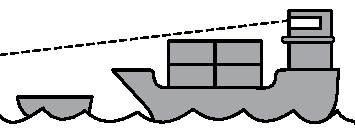
\includegraphics[width=\textwidth]{Hoofdstukken/Veiligheid/pdf/dode_hoek.pdf}
        \caption{Dode hoek}
        \label{pic:dodehoek}
    \end{figure}
  \end{minipage}
    \hspace{2cm}
  \begin{minipage}[b]{0.32\textwidth}
  \begin{figure}[H]
 		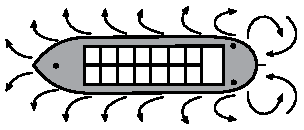
\includegraphics[width=\textwidth]{Hoofdstukken/Veiligheid/pdf/zuiging.pdf}
        \caption{Zuiging}
        \label{pic:zuiging}
    \end{figure}
  \end{minipage}
  \end{center}


\subsection{Diepgang  \hfill \textit{Figuur \ref{pic:diepgang}}}
Veel wateren hebben een vaargeul, dit is een dieper deel van het vaarwater. Soms is dit aangegeven met boeien of tonnen. Grote boten die zwaar beladen zijn kunnen soms alleen in dit deel van het water varen. Ze zullen misschien niet kunnen wijken voor je en jij zal daar rekening mee moeten houden.

\subsection{Verlijeren  \hfill \textit{Figuur \ref{pic:verlijeren}}}
Net als bij een zeilboot, kunnen ook grote motorschepen verlijeren. Als de wind van de zijkant komt, zal deze het schip opzij duwen. Om dit te corrigeren zal hij een beetje schuin gaan varen. Dit zorgt ervoor dat hij meer ruimte inneemt en minder wendbaar is. Geef deze schepen de ruimte. 

  \begin{center}
  \begin{minipage}[b]{0.30\textwidth}
    \begin{figure}[H]
        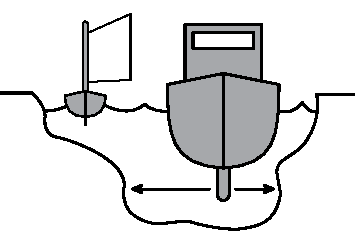
\includegraphics[width=\textwidth]{Hoofdstukken/Veiligheid/pdf/diepgang.pdf}
        \caption{Diepgang}
        \label{pic:diepgang}
    \end{figure}
  \end{minipage}
    \hspace{2cm}
  \begin{minipage}[b]{0.25\textwidth}
  \begin{figure}[H]
        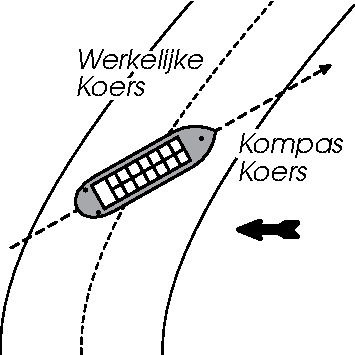
\includegraphics[width=\textwidth]{Hoofdstukken/Veiligheid/pdf/verlijeren.pdf}
        \caption{Verlijeren}
        \label{pic:verlijeren}
    \end{figure}
  \end{minipage}
  \end{center}


\section{Conclusie}
Je hebt in dit hoofdstuk geleerd wat belangrijk is om veilig te zeilen. Zo zijn er regels voor reddingsvesten, een gedragscode en is het slim om goed op het weer te letten - zowel voor als tijdens het varen. Als laatst is er nog gekeken naar vaarproblemen bij andere, voornamelijk grote, schepen.